\documentclass[AMS, Times1COL]{article} %STIX1COL,STIX2COL,STIXSMALL
\usepackage[margin=0.75in]{geometry}
\usepackage{graphicx}
\usepackage{pgfplots}
\usepackage{pgfpages}
\usepackage{listings}
\usepackage{makecell}
\usepackage{subfiles}
\usepackage{hyperref}
\usepackage{hyphenat}
\usepackage{amsmath}
\usepackage{amssymb}
\usepackage{amsthm}
\usepackage{authblk}
\usepackage{comment}
\usepackage{tikz}
%\usepackage{algpseudocode}
%\usepackage{caption}
\usepackage{tkz-berge}
\usepackage{subcaption}
\usepackage{xr}
\usepackage{setspace}
\usepackage{hyperref}
\usepackage{tabularx}
\usepackage{listings}
\usepackage{booktabs}
\usepackage[utf8]{inputenc}
\usepackage{hyperref}
\usetikzlibrary{fit} % Load the library
\usetikzlibrary{positioning, fit, shapes.geometric, arrows.meta}
\usetikzlibrary{calc}
\usetikzlibrary{shapes.geometric, arrows.meta, positioning}
\usetikzlibrary{bending}
\usetikzlibrary{shapes, arrows.meta, graphs, quotes}
\usetikzlibrary{patterns.meta}
\raggedbottom
\tikzstyle{startstop} = [rectangle, rounded corners, minimum width=3cm, minimum height=1cm,text centered, draw=black, fill=blue!20]
\tikzstyle{process} = [rectangle, minimum width=3.5cm, minimum height=1cm, text centered, draw=black, fill=orange!30]
\tikzstyle{decision} = [diamond, aspect=2, minimum height=1.2cm, text centered, draw=black, fill=green!30]
\tikzstyle{arrow} = [thick,->,>=stealth]
\newtheorem{exmp}{Example}[section]
\newtheorem{theorem}{Theorem}[section]
\newtheorem{lemma}[theorem]{Lemma}
\newtheorem{proposition}[theorem]{Proposition}
\newtheorem{corollary}[theorem]{Corollary}
\newtheorem{conjecture}[theorem]{Conjecture}
\theoremstyle{definition}
\newtheorem{definition}{Definition}[section]
\newtheorem{example}{Example}[section]
\newtheorem{exercise}{Exercise}[section]
\newtheorem{remark}{Remark}[section]
\geometry{margin=0.75in}
\newcommand{\email}[1]{\def\@email{#1}}
\newcommand{\keywords}[1]{\def\@keywords{#1}}
\newcommand{\address}[1]{\def\@address{#1}}
\title{A Minimum Counterexample Proof of the Seymour Second Neighborhood Conjecture via the Graph Level Order}
\pgfplotsset{compat=1.18}
\begin{document}
	\author{Charles N. Glover}
	\affil{Washington, DC \\\texttt{cnglover@umd.edu}}
	
	\keywords{oriented graphs, minimum counterexample, breadth-first search, minimum out-degree node, set theory}
	\maketitle
	
	\abstract{We provide a constructive proof of the **maximal set version** of the Seymour Second Neighborhood Conjecture (SSNC) by reframing the problem as a set-packing optimization problem. The universal family of oriented graphs $\mathcal{O}$ is classified by their minimum out-degree $\delta$. This shifts the objective to maximizing the number of non-Seymour vertices.

A counterexample is a packing of vertices that fail the SSNC. To prove such a packing is unsustainable, we introduce the Graph Level Order (GLOVER). This BFS-based coordinate system partitions $\mathcal{O}$ into rooted neighborhoods $R_i$ from a minimum out-degree node.

Set-theoretic multiple parents resolve the double-counting that has plagued Seymour diamonds. This coordinate system also categorizes transitive triangles into eight distinct types and proves that seven are inconsistent in an MCE environment.

Distinguishing it from standard BFS, the dual MCE metric first minimizes the number of interior neighbors, then maximizes total interior degree. This environment forces cycles in the first neighborhood of every parent, causing neighborhoods to become quadratically dense as they both decrease in size and demand more arcs.

The proof concludes with a supply-demand collision. Arc capacity is consumed when $i > \frac{\delta}{3}$, making the packing of non-Seymour vertices unsustainable. Consequently, the appearance of a Seymour set of vertices is forced in every MCE. The algorithm to identify these vertices runs in $O(\vert{}V\vert{}+\vert{}E\vert{})$ time, confirming its capability to operate on large, dense oriented networks in polynomial time.
	}
	
	
	\section{Introduction}\label{intr}
	
	The Seymour Second Neighborhood Conjecture (SSNC), proposed in 1990, remains a famously stubborn problem in graph theory. It asks if every oriented graph contains a vertex whose second out-neighborhood is at least as large as its first. We prove this conjecture by analyzing the universal family of oriented graphs $\mathcal(O)$. Our solution introduces the Graph Level Order. This is a coordinate system that organizes vertices by minimum out-degree $\delta$. This framework also provides an efficient algorithm for identifying the vertex.
	
	\begin{conjecture}\label{nbconj}
		(Seymour's Second Neighborhood Conjecture (SSNC)). For every oriented graph $G \in \mathcal{O}$, there exists a vertex $v \in V(G)$ such that $|N^{++}(v)| \geq |N^+(v)|$. The sets $N^+(v)$ and $N^{++}(v)$ denote the first and second out-neighborhoods of $v$, respectively.
	\end{conjecture}
	
	This conjecture was first published by Nate Dean and Brenda Latka in 1995 \cite{DL}. They proposed a related version for tournaments, which are complete oriented graphs. The tournament case was proved by Fisher \cite{F} in 1996, with an alternative proof later provided by Havet and Thomassé \cite{HT} in 2000.
	
	Fisher's approach \cite{F} proved a vertex exists but offered no way to locate it. By using Farkas' Lemma, he showed the conjecture holds. Havet and Thomassé \cite{HT} advanced the problem with median orders. These are linear orderings that minimize the number of back arcs. Their proof identifies the last vertex of a median order as the one satisfying the Dean Conjecture. Finding median orders is NP-hard, but Havet and Thomassé only needed to know that such an ordering exists. This allowed them to speak of it without finding it. This became a powerful tool in tournament theory.
	
	While this inductive approach resolved the Dean Tournament Conjecture, it relies on the completeness of tournaments. The technique fails to generalize to all oriented graphs. Non-adjacent vertices give median orders no restrictions on how to order vertices because both orderings result in zero back arcs for the pair. This makes this approach ineffective as density decreases.
	
	Kaneko and Locke \cite{KL} showed the SSNC holds for graphs with a minimum degree of at most six. This work serves as a foundation for much research on the SSNC. However, it introduced another NP-hard problem, dominating sets, into the SSNC. For cases greater than six, the complexity was too high to solve efficiently.
	
	Chen et al. \cite{CS} established a lower bound for the SSNC. They demonstrated that a vertex meets a relaxed version of the condition. This work was extended by Huang and Peng \cite{HP}. These researchers used Constraint Satisfaction Programming (CSP) to find variable assignments that satisfy the conjecture. This is a method that frames the SSNC as logical constraints to be satisfied and optimized using SAT solvers.
	
	Recent work by Diaz et al. \cite{Di}, extending Bottler et al. \cite{BMN}, confirms that almost all random graphs $G(n, p)$ satisfy the conjecture. By analyzing binomial random graphs with random orientations, they show that Seymour vertices are statistically typical. This provides a valuable average-case perspective, even if the worst-case proof remains out of reach. Botler et al. use shortest paths to define neighborhoods, which performed well for analyzing pseudo-random orientations on a global scale.
	
	However, identifying Seymour vertices in random graphs reveals nothing about the internal properties that guarantee the conjecture's truth. Fundamental questions remain: How do connectivity, degree distribution, and neighborhood growth force the existence of these vertices?
	
	The CSP framework and random graph models provide valuable existence proofs. Still, they face limitations when addressing the general conjecture. These models typically treat the graph as a field of quasi-independent variables. More accurately, an oriented graph can be described as an iterated sequence of dependencies. The work of Botler et al. is foundational in its analysis of pseudo-random orientations. Yet, this neighborhood system operates through local, relative distances. This creates an unanchored topological space where every node is a potential origin.
	
	If Seymour vertices prove to be universal within the class $\mathcal{O}$, both these approaches suffer from a lack of causality. The graph class will always satisfy the constraints imposed. As a result, these models confirm the existence of the property without discovering the reasons why. They observe the result of the law without defining the law itself.
	
	Diaz et al. \cite{Di} do explore the contrapositive of the Seymour conjecture. Propositions 4 and 5 show that if the conjecture were false, infinitely many strongly connected graphs with bounded minimum out-degrees lack Seymour vertices. This reasoning mirrors our minimum counterexample. Diaz et al. do not explicitly define non-Seymour vertices. Their counterexample modeling shares the same motivation.
	
	Lladó \cite{Llado2013} proved the conjecture for highly connected regular digraphs, showing that any counterexample would violate the basic properties of regularity. Her proof uses Menger's theorem to bound neighborhood sizes. This approach is bounded by the regularity assumption; without it, the method cannot be extended to broader graph classes.
	
	Brantner et al. \cite{BBKS} introduced two key configurations: transitive triangles and Seymour diamonds. A transitive triangle—where two edges from different sources share a destination—creates a shortcut in reachability. A Seymour diamond consists of four edges that split from a common source and converge at a shared target. Brantner et al. proved that any graph without transitive triangles must contain a Seymour vertex, suggesting these triangles are a primary obstacle to the conjecture.
	
	This work extends to $m$-free, $k$-transitive, and $k$-anti-transitive graphs. An $m$-free graph contains no directed cycles of length $m$ or less. Daamouch \cite{Da} showed that certain shortcuts—specifically $k$-transitive graphs (for $k \leq 6$) and $k$-anti-transitive graphs (for $k \leq 4$)—guarantee a Seymour vertex. Hassan et al. \cite{HKPS} later extended these results to include 6-anti-transitive graphs.
	
	Other researchers have tested the conjecture on tournaments missing specific substructures. Fidler and Yuster \cite{FidlerYuster} confirmed it for tournaments missing a star or multiple edges from a single node, a result Ghazal \cite{Ghazal_2011} later reinforced. Similarly, Mniny and Ghazal \cite{MninyGhazal} proved the conjecture for oriented graphs missing configurations like $C_4$, the chair, or the co-chair. Most recently, Daamouch et al. \cite{daamouch2024secondneighborhoodconjecturetournaments} extended this to tournaments missing two stars or disjoint paths.
	
	Transitive triangles complicate the conjecture because first neighbors seem to steal counts from second neighbors. Here, degree and distance conflict: one arc increases the degree of a vertex, while one path defines distance. Resolving the conjecture requires mastering this interaction between degree and distance, particularly within these triangular structures.
	
	Another approach uses subset-level expansion bounds to restrict the behavior of potential counterexamples. Seacrest \cite{Scrt} used neighborhood ratios across subsets rather than individual nodes. This showed that a hypothetical minimum counterexample could be bounded in size to at most $\binom{\delta +1}{2}$ vertices, where $\delta$ is the minimum out-degree. The problem with this approach is that out proves facts about average neighborhood expansion. However, the SSNC seeks a single vertex whose degree doubles. Bridging the gap between average subset behavior and the existence of a single vertex remains a major challenge.
	
	In a 2021 poster, Illia Nalyvaiko \cite{NALYVAIKO2021poster} explored the conjecture's contrapositive. He introduced a penalty function to evaluate potential counterexamples. His intuition differs from non-Seymour vertices. Both approaches shift the focus from verifying the conjecture to testing its bounds. Nalyvaiko's method offered a novel perspective that aligns with our motivations.
	
	\begin{tabular}{|l|l|l|}
		\hline
		\textbf{Method} & \textbf{Core Strength} & \textbf{Limitation for SSNC}\\
		\hline
		BFS & Rooted Traversal & Produces trees; lacks cycles to bound $N^{++}$ \\
		\hline
		Median Orders & Effective for Tournaments & Dependent on high edge density; NP-Hard\\
		\hline
		CSP & Local Verification & Treats nodes as independent; no global logic \\
		\hline
		Random Graphs & Statistical Modeling & ``Unanchored'' nodes; lacks a fixed origin \\
		\hline
	\end{tabular}
	
	We provide an algorithmic construction to identify the target node and demonstrate its structural consistency. To ensure testability and reproducibility, implementations in Python and interactive visualizations in JavaScript are publicly available on \href{https://github.com/Cgcharles7/ssnc
	}{GitHub}.
	
	Prior work focused on proving existence in special cases or identifying missing substructures. These approaches, while foundational, offered no way to actually find a Seymour vertex. The Graph Level Order organizes the oriented graph space $\mathcal{O}$ into rooted neighborhoods based on distance from a minimum out-degree vertex $\delta$. When combined with the negation of the conjecture, this method identifies set-theoretic relationships forcing cycles to exist, leading to a path to a Seymour vertex. This framework transforms the conjecture from an existential puzzle into a constructive set packing problem. It enables the linear-time identification of nodes and unifyies decades of disparate research.
	
	This paper presents our methodology, supported by lemmas and examples. A novel data structure is then introduced to tackle the conjecture's core challenges and show how it integrates with maximizing non-Seymour nodes. After proving our main theorem and analyzing the algorithm's complexity, we conclude with future research directions.
	
	\section{Exploring the Minimum Counterexample}\label{cont}
	
	Graph theory is the study of relationships. The Graph Level Order introduces set-theoretic ancestry to those connections. After identifying the limitations of existing terminology, we formally define the Graph Level Order architecture. This includes new set-theoretic types of neighbors, partitions of those neighbors, and theorems mapping these terms to existing terminology. This systematic reorganization provides the clarity necessary to resolve the SSNC.
	
	A Seymour node is a node satisfying the conjecture. Consequently, a non-Seymour node is the node-level negation of the SSNC, requiring a strict inequality ($|N^{++}(u)| < |N^{+}(u)|$). The objective is to maximize the number of non-Seymour vertices inside a graph $G \in \mathcal{C}$ (the set of counterexamples).
	
	If any node fails to be non-Seymour, it proves the conjecture. As a result, these non-Seymour nodes work in unison towards not allowing a Seymour vertex.
	
	Most researchers who work on this problem use shortest paths to distinguish first neighbors from second. The Breadth-First Search (BFS) algorithm extends that concept to entire graphs. When a second metric of lexicographic ordering is added to distinguish nodes at the same distance, this becomes a well-ordering of vertices.
	
	\begin{theorem}[BFS-Lex Coordinate System]\label{bfslex}
		For any finite, connected oriented graph $G \in \mathcal{O}$ and root vertex $v_0 \in V(G)$, there exists a unique Well-Ordering of V(G) induced by a breadth-first search (BFS) algorithm combined with a lexicographical tie-breaking rule.
	\end{theorem}
	
	This well ordering can easily be seen by a mapping from the coordinate pair of a node's BFS distance and lexicographic ID to the natural numbers. 
	
	Standard neighborhood definitions suffer from an accounting failure: they cannot be partitioned without destroying ancestral data. When a node's influence is sent to its first neighbors, the connection to its second neighbors is reduced to a simple count. This strips distance-two neighbors of any knowledge of their ancestry. This loss creates a disconnect and makes it impossible to track the precise distribution of out-degree influence.
	
	This counting problem is demonstrated in the following case:
	
	Let $u_i$ be a parent node, and let $v_{i+1}, w_{i+1} \in N^+(u_i)$ be distinct children of $u_i$. Suppose there exists a vertex $y_{i+2}$ such that $$ v_{i+1} \to y_{i+2} \in G \quad \text{and} \quad w_{i+1} \to y_{i+2} \in G, \text{ but } u_i \not\to y_{i+2} \in G. $$ Then the quadruple $(u_i, v_{i+1}, w_{i+1}, y_{i+2})$ forms a \textbf{Seymour diamond}.
	
	\begin{figure}[ht]
		\centering
		\begin{tikzpicture}[node distance=2cm]
			\node (u_i) at (0, 0) {$u_i$};
			\node (v_{i+1}) at (2, 2) {$v_{i+1}$};
			\node (w_{i+1}) at (2, -2) {$w_{i+1}$};
			\node (y_{i+2}) at (4, 0) {$y_{i+2}$};
			\draw[->][thick] (u_i) -- (v_{i+1});
			\draw [->](u_i) -- (w_{i+1});
			\draw[->][thick] (v_{i+1}) -- (y_{i+2});
			\draw [->](w_{i+1}) -- (y_{i+2});
			
		\end{tikzpicture}
		\caption{\textit{\textbf{A Seymour diamond}. A parent node $u_{i}$ with children $v_{i+1}$ and $w_{i+1}$, and a shared grandchild $y_{i+2}$ resulting in double counting in neighborhood analysis. The sum of the children's out-degrees is $|N^{+}(v_{i+1})|+|N^{+}(w_{i+1})|$. The actual contribution to the second out-neighborhood $|N^{++}(u_{i})|$ is only one, as both arcs terminate at the same node, $y_{i+2}$.} }
		\label{smdmpic}
	\end{figure}
	
	Seymour diamonds double-count second neighbors.
	When two children at distance one, $v_{i+1}$ and $w_{i+1}$, both point to the same node $y_{i+2}$, a summation of their out-degrees fails. The operation $|N^+(v_{i+1})| + |N^+(w_{i+1})|$ incorrectly counts the same node twice.
	
	\begin{remark}{Why New Definitions Are Needed}
		Standard neighborhoods $N^+(v)$ and $N^{++}(v)$ discard layer-ancestry information, causing the Seymour diamond double-counting problem. When two children of the same parent both point to the same grandchild, summing their out-degrees counts that grandchild twice. The canonical partition presents positional data and makes the double-counting resolvable. The second neighborhood is a union of forward neighbor sets, not a sum. 
	\end{remark}
	
	The \textbf{rooted neighborhood} at distance $i \ge 0$ from $v_0$ is the subgraph induced by the vertices at directed distance $i$ from $v_0$.
	
	A triple of vertices $x,y,u$ in an oriented graph $G$ forms a \textbf{transitive triangle} if $$ x \to y,\qquad x \to u,\qquad y \to u, $$ i.e., the three vertices induce an acyclic orientation of a 3-cycle.
	
	Let $u_i \in R_i$ be a parent node in the rooted layering, and let $v_{i+1} \in R_{i+1}$ be one of its children. The \textbf{interior neighbors} of $v_{i+1}$ with respect to $u_i$ are the vertices $$ \text{int}(u_i, v_{i+1}) = N^+(u_i) \cap N^+(v_{i+1}). $$ The \textbf{interior degree} of $v_{i+1}$ with respect to $u_i$ is $$ |\text{int}(u_i, v_{i+1})|. \label{int_nbr} $$
	
	Let $u_i \in R_i$ be a parent of $v_{i+1} \in R_{i+1}$. The \textbf{exterior neighbors} of $v_{i+1}$ with respect to $u_i$ are the vertices $$ \text{ext}(u_i,v_{i+1}) = N^{++}(u) \cap N^+(v_{i+1}). $$
	The \textbf{exterior degree} of $v_{i+1}$ with respect to $u_i$ is $$ |\text{ext}(u_i, v_{i+1})|. $$\label{ext_nbr}
		
	\begin{remark} For the MDN $v_0$, all its out-neighbors are exterior neighbors because $R_0 = \{v_0\}$ and there are no earlier neighborhoods $R_{-1}$. Thus, $$ \text{int}(v_0, v) = \emptyset \hspace{1cm} \forall v \in\space R_1 $$ \end{remark}
	
	Let $v_0$ be the MDN, and let $u_i \to v_{i+1} \in G$, with $u_i \in R_i$ and $v_{i+1} \in R_{i+1}$. The set of \textbf{back neighbors} from $v_i$ is $\text{back}(v_{j})$. The set of all back neighbors of $u_i$ is denoted $\bigcup_{j <= i} R_j \text{back}(u_i)$. \label{back_def} 
	
	Back neighbors are a well studied problem in graph theory and this definition is consistent with literature. To assist with solving the SSNC, we will partition the set of back neighbors further: connected and disconnected back neighbors. 
	
	Given a parent-child arc $u \to v$ where $u \in R_i$ and $v \in R_{i+1}$, an outgoing arc from $v$ to a target vertex $w$, denoted as $u \to v \to w$, is classified as \textbf{connected back neighbors} if the target vertex $w$ resides in the immediately preceding adjacent layer. \label{conn_back_def}
	
	Given a parent-child arc $u \to v$ where $u \in R_i$ and $v \in R_{i+1}$, an outgoing arc from $v$ to a target vertex $w$, denoted as $u \to v \to w$, is classified as \textbf{disconnected back neighbors} if the target vertex $w$ resides in an earlier layer that is separated by at least one intermediate layer. Disconnected back neighbors bypass at least one layer. \label{disc_back_def}
	
	This is a minimum counterexample approach to the SSNC. Let $G \in \mathcal{O}$ be an oriented graph. Let $\mathcal{C}$ be the (possibly empty) set of all counterexamples to SSNC. Let $G \in \mathcal{C}$ be a counterexample. Let $\omega$ be a BFS-Lex well-ordering $G$ rooted at its minimum out-degree node $v_0$. For a fixed integer $k$, let $G_k$ denote the induced subgraph consisting of the first $k$ vertices of $G$ under the ordering $\omega$. The graph $G \in \mathcal{C}$ is a \textbf{Minimum Counterexample (MCE)} if it is constructed using the BFS-Lex algorithm rooted at a minimum out-degree node $v_0$ and which also minimizes the interior neighbors and the maximum total interior degree in each layer. 	
	
	\begin{definition}\label{glover1}
		Let $G = (V,E)$ be an oriented graph represented by an MCE, and let $v_0 \in V$ be the vertex of minimum out-degree. A \textbf{Graph Level Order} on $G$ consists of the following structure:
		\begin{enumerate}
			\item Well Ordered Rooted Neighborhoods: Partition the vertices of $V$ into rooted neighborhoods $$R_i=\{v \in V : \text{dist}(v_0,v)=i\}, \text{ for } i=0,1,\dots,n.$$
			\item Well Ordered Vertices: For vertices $u_{i,k_1}, u_{i,k_2} \in R_i$ and $v_{j,m_1}, v_{j,m_2} \in R_j$ with $i<j$, we have $u_{i,k_1}, u_{i,k_2}<v_{j,m_1}, v_{j,m_2}$ and $u_{i,k_1} < u_{i,k_2}$.			
			\item Ancestry-Awareness: For each parent-child pair $u_i \to v_{i+1}$ with $u_i \in R_i$ and $v_{i+1} \in R_{i+1}$, the out-neighbors of $v_{i+1}$ are classified into the three disjoint sets according to Lemma \ref{nodepartition}: $\text{back}(u_i, v_{i+1})$, $\text{int}(u_i,v_{i+1})$, and $\text{ext}(u_i,v_{i+1})$.
		\end{enumerate}
	\end{definition}

Prior SSNC efforts have largely followed two methodologies: One considers transitive triangles as building blocks to be leveraged \cite{FidlerYuster, MninyGhazal, Ghazal_2011, daamouch2024secondneighborhoodconjecturetournaments}, while the other think they should be ignored across a class of problems \cite{Da, HKPS, BBKS}. Our BFS layering approach moves beyond this binary of requiring or forbidding transitivity. By partitioning the graph, we isolate the influence of these triangles based on their inter-layer distribution. Forward-facing transitive triangles serve as a type that can enforce a non-decreasing neighborhood condition.
		
	This MCE will be constructed under the BFS-lex well-ordering on $V(G)$. This will be modeled through an iterative packing process. At any step $k$, the vertex set $V(G)$ is partitioned into a vector of three distinct, mutually exclusive zones:
	
	\begin{itemize}
		\item Passed: These vertices have successfully achieved their non-Seymour status.
		
		\item Active: These vertices are actively being processed and their out-arcs might prevent a node from becoming non-Seymour.
		
		\item Upcoming: These are the second and later neighbors of the proven non-Seymour nodes.
	\end{itemize}
	
	Prior SSNC efforts have largely followed two methodologies: One considers transitive triangles as building blocks to be leveraged \cite{FidlerYuster, MninyGhazal, Ghazal_2011, daamouch2024secondneighborhoodconjecturetournaments}, 
		
	\section{No Back Neighbors}
	
	When an MCE contains no back arcs, the vertex out-degree is strictly partitioned between forward/interior and exterior directions.
	
	\begin{lemma}[Degree Partition]\label{nodepartition}
		Let $u_i \in R_i$ and let $v_{i+1} \in R_{i+1}$ be vertices of an MCE, with $u_i \to v_{i+1} \in G$. Then the out-neighborhood of $v_{i+1}$ admits the disjoint partition
		
		$$N^+(v_{i+1}) = \text{int}( u_i, v_{i+1}) \;\dot{\cup}\; \text{ext}( u_i, v_{i+1}).$$ \end{lemma}
	\begin{proof}
		Every out-neighbor of $ v_{i+1}$ lies in exactly one rooted neighborhood.
		Arcs may point only to vertices in layers $R_{i}$, $R_{i+1}$, or $R_{i+2}$.
		Thus any $x \in N^+( v_{i+1})$ lies in one of these layers.
		\begin{description}
			\item If $x \in R_{i+2}$, then $x \in \text{ext}( u_i, v_{i+1})$.
			\item If $x \in R_{i+1}$, then $x \in \text{int}( u_i, v_{i+1})$. 
		\end{description}
		These sets are disjoint because distance is disjoint and cover all of $N^+( v_{i+1})$.
	\end{proof}

The assumption of no back neighbors simplifies our analysis. As we will see, the BFS traversal reveals many types of transitive triangles. The exclusion of back neighbors from this case means that the only remaining ones are the forward facing transitive triangles and same layer transitive triangles. These forward facing transitive triangles are what were defined as interior neighbors and help to keep a parent node non-Seymour. 
	
	\begin{theorem} (Neighborhood Size). Let $G \in \mathcal{O}$ be be an MCE with MDN $v_0$, with rooted neighborhoods $R_0$, $R_1$, $\ldots$, $R_k$ constructed by the BFS. Suppose all nodes are non-Seymour. Then for all $i \geq 0$, $R_k| = \delta - k + 1$. 
	\end{theorem} \label{layer_size}
	
	\begin{proof}
		We proceed by induction on $i$. 
		Base Case ($i = 0$): 
		The root $R_0$ = $\{v_0\}$ has out-neighbors $R_1 = N^+(v_0)$. Consider $v_1 \in R_1$. If $v_1$ has more than $\delta$ exterior neighbors, then the node $v_0$ will be a Seymour node. The pigeonhole principle then forces $v_1$ to have at least one interior neighbor. If $v_1$ has more than one interior neighbor, then the subgraph $R_1$ violates the minimum neighborhood density metric, and thus $G$ would not be an MCE. This forces $v_1$ to have exactly 1 interior arc and $\delta - 1$ exterior arcs. 
		
		Induction Hypothesis: Assume that for some $i \geq 0$, $|R_k| = \delta - k + 1$.
		
		Inductive Step: Consider $u_{k} \in R_{k}$ and $v_{i+1} \in R_{i+1}$ with $u_{i} \to v_{i} \in G$. 
		By the I.H., we know that $|R_k| = \delta - k + 1$. If $v$ were to send more than $\delta - k + 1$ exterior neighbors to $R_{k+1}$, this would make $u_k$ Seymour. As a result, $v_{k+1}$ must have at least $k+1$ interior neighbors. Thus, by the partition lemma, this allows $v_{k+1}$ to only send $\delta - (k+1)$ nodes to $R_{k+2}$. 
		
		Similar to case 1, if $v_{k+1}$ sent too few nodes to $R_{k+2}$, this would result in $v_{k+1}$ having more interior arcs than required, and $G$ violating the minimum neighborhood density requirement for an MCE. 
		
		Thus, the bound holds at level $i + 1$ and by induction, the statement is true for all $i \geq 0$.
	\end{proof}
	
	\begin{figure}
	\centering
	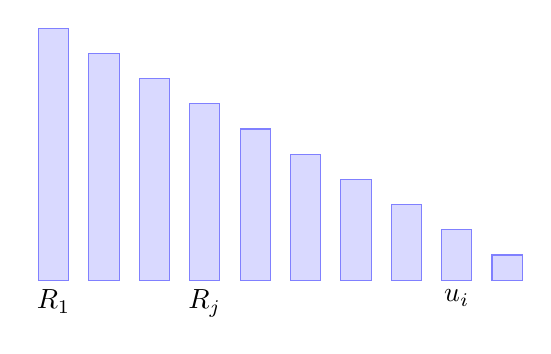
\begin{tikzpicture}[x=0.8cm, y=0.4cm, scale=0.8]
		% Loop to draw 10 bars (shortened for clarity), decreasing in height
		\foreach \h [count=\i] in {10, 9, 8, 7, 6, 5, 4, 3, 2, 1} {
			% Draw vertical bar
			\draw[fill=blue!15, draw=blue!50] (\i, 0) rectangle (\i+0.6, \h);
			
			% Label the levels
			\ifnum\i=1 \node[below] at (\i+0.3, 0) {$R_1$}; \fi
			\ifnum\i=4 \node[below] at (\i+0.3, 0) {$R_j$}; \fi
			\ifnum\i=9 \node[below] at (\i+0.3, 0) {$u_i$}; \fi
		}
	\end{tikzpicture}
	\caption{\textit{\textbf{Iterated decrease in second neighborhood}. In a rooted environment, this means that there is a maximum value that every decrease comes from: $|R_k| = \delta - (k-1)$}}
	\end{figure}

The neighborhood size requires a number of nodes in each layer. These layers decrease in size with distance. This implies that as layers move further from the root, the nodes within the layers will need to make more intra-layer connections to meet their minimum out-degree requirements. 
	
	\begin{theorem}
	Let $G\in \mathcal{O}$ be an MCE represented by rooted neighborhoods $R_0, R_1, \ldots, R_n$. Further, let each $R_i$ have the size $|R_i| = \delta - i + 1$. For each node $u_i \in R_i$ we also have that without back arcs its nodes can be partitioned into interior and exterior neighbors. Then we have that $\text{int}(u, v) \ge k + 1$ for $u \in R_i$, $v \in R_{k+1}$, and $u \to v \in G$. 
	\end{theorem}
	\begin{proof}
	Let $v_{k+1} \in R_{k+1}$ be a child of $u_k \in R_k$. 
	By Theorem \ref{layer_size} we know that at least $\delta - (k+1) + 1$ nodes are necessary in $R_{k+1}$ to keep $u_k$ from being Seymour. 
	By the pigeonhole principle, to keep $u_k$ non-Seymour, the node $v_{k+1}$ must have no more than $delta - (k+2) + 1$ exterior arcs. 
	\end{proof}

Another consequence of the rooted neighborhood size formula is that it sets the worse possible rate of decrease. The lower bound for interior neighbors is also an upper bound for exterior neighbors (because there are no back neighbors). 
		
	\begin{lemma}[Extra Forward Arc Produces Seymour Vertex]
		Let $G$ be an MCE without back arcs with unique node coordinates. Let $u, v \in V(G)$ be nodes such that $v$ is in the adjacent forward layer ($\text{dist}(v) = \text{dist}(u) + 1$), and let $(u, v)$ be a forward arc in $G$. 
		
		If the number of exterior neighbors associated with $(u, v)$ bounds $u$'s out-degree from below, i.e.,
		$$|N^+(u)| \le |\text{ext}(u, v)|$$
		then $u$ satisfies the Seymour second neighborhood condition:
		
		$$|N^+(u)| \le |N^{++}(u)|$$
		
	\end{lemma}
	
	\begin{proof}
		Let $c \in \text{ext}(u, v)$ be an arbitrary exterior neighbor of $u$ relative to $v$. 
		By definition of exterior neighbors in $G$, $c$ is reachable from $u$ via a directed path of length 2 passing through $v$. Thus, every exterior neighbor $c$ belongs to the second neighborhood $N^{++}(u)$, giving the set inclusion:
		\[
		\text{ext}(u, v) \subseteq N^{++}(u)
		\]
		
		Taking the cardinalities of both finite sets, set inclusion implies:
		\begin{equation}
			|\text{ext}(u, v)| \le |N^{++}(u)|
		\end{equation}
		
		By hypothesis, we are given that the first neighborhood of $u$ is bounded by the exterior neighbors:
		\begin{equation}
			|N^+(u)| \le |\text{ext}(u, v)|
		\end{equation}
		
		Combining inequalities (2) and (1) by the transitivity of inequality on $\mathbb{N}$:
		
		$$|N^+(u)| \le |\text{ext}(u, v)| \le |N^{++}(u)| \implies |N^+(u)| \le |N^{++}(u)|$$
		
		This proves that $u$ is a Seymour vertex.
	\end{proof}
	
		\begin{lemma}[MCE Interior Degree]\label{intdeg}
		Let $G \in mathcal{O}$ be a counterexample. Suppose $u_k \in R_k \to v_{k+1} \in R_{k+1}$ is a parent child pair. Let $\text{int}(u_k, v_{k+1})$ represent its interior degree, then:
			
			$$\text{int}(u, v) = k$$
	\end{lemma}
	\begin{proof}
		Suppose for the sake of contradiction that the interior degree strictly exceeded the layer distance:
		
		$$int(u, v)>k$$
By MCE and non-Seymour constraints, an interior degree greater than $k$ is over-connected. 
This violates the MCE and is thus not minimal. 
		
Because assuming $\text{int}(u, v) > k$ leads to a violation of the MCE hypothesis, this case is impossible.

Therefore, by elimination of the upper violation, the interior degree is bounded by $k$:
		$$\text{int}(u, v) = k$$
		
	\end{proof}
	
	\section{Disconnected Back Neighbors}
	
	To prevent parents from becoming Seymour vertices, neighborhood sizes must contract strictly as distance increases. This imposes strict constraints on interior and exterior arc allocation:
	
	If a node possesses an excess forward arc bypassing the immediate next neighborhood layer, it prematurely populates the second out-neighborhood, forcing $\vert{}N^{++}(u)\vert{} \ge \vert{}N^{+}(u)\vert{}$ and immediately creating a Seymour vertex.
	If a node takes on too many interior arcs, it exceeds the local density threshold of the subgraph $R_i$, violating the minimum counterexample's density minimization condition.
	If interior arc counts drop below the required threshold, the vertex fails to constrain its second neighborhood through local cycle packing, forcing extra forward arcs that trigger the Seymour condition.
		
	\begin{lemma}[Seymour Property under Disjoint Back Arcs]
		Let $G$ be a graph represented by an MCE, and let $a, b \in V(G)$ such that $b \in N^+(a)$. If the out-neighbors are completely disjoint ($N^+(b) \cap N^+(a) = \emptyset$), $b$'s out-neighborhood contains no duplicates, and the degree bounds satisfy $|N^+(a)| \le \delta \le |N^+(b)|$, then $a$ satisfies Seymour's condition:*
		
		$$|N^1(a)| \le |N^2(a)|$$
	\end{lemma}\label{no_disj}
	\begin{proof}
		By definition, the first neighborhood $N^1(a)$ is a subset of $a$'s out-neighbor list:
		
		$$|N^1(a)| \le |N^+(a)|$$
		
		We claim that every vertex $z \in N^+(b)$ belongs to the second neighborhood $N^2(a)$. To verify this, let $z \in N^+(b)$. By definition:
		\begin{itemize}
			\item $z$ is reachable from $a$ in two steps via the path $a \to b \to z$ (since $b \in N^+(a)$ and $z \in N^+(b)$).
			\item $z \neq a$, because $a \notin N^+(b)$ (anti-symmetry constraint).
			\item $z \notin N^+(a)$, because $N^+(b) \cap N^+(a) = \emptyset$.
		\end{itemize}
		
		Since $b$'s out-neighborhood contains no duplicates, its size as a set matches its list length:
		
		$$|N^+(b)| = |^+(b)|_{\text{set}}$$
		
		Because $N^+(b) \subseteq N^2(a)$, it follows directly that:
		
		$$|N^+(b)| \le |N^2(a)|$$
		
		Combining our bounds with the minimality and regularity conditions ($|N^+(a)| \le \delta \le |N^+(b)|$), we chain the inequalities:
		
		$$|N^1(a)| \le |N^+(a)| \le \delta \le |N^+(b)| \le |N^2(a)|$$
		
		Therefore, $|N^1(a)| \le |N^2(a)|$, completing the proof. 
	\end{proof}		
				
	\begin{lemma}[Termination of Disconnected Chains]
		Let $\alpha$ be a type, let $\mu: \alpha \to \mathbb{N}$ be a measure function, and let $P$ and $\text{Closes}$ be predicates on $\alpha$. 
		If $P$ holds for at least one element, and for every element $a$ satisfying $P(a)$, either $\text{Closes}(a)$ holds or there exists a successor $b$ such that $P(b)$ holds and $\mu(b) < \mu(a)$, then there exists an element satisfying both $P$ and $\text{Closes}$.
		
		$$\left(\exists a, P(a)\right) \land \left(\forall a, P(a) \implies \text{Closes}(a) \lor \exists b, P(b) \land \mu(b) < \mu(a)\right) \implies \exists a, P(a) \land \text{Closes}(a)$$
	\end{lemma}\label{no_cbain}
	\begin{proof}
		By the well-foundedness of the natural numbers under strict inequality ($\langle \mathbb{N}, < \rangle$ is well-founded), any non-empty subset of $\alpha$ mapped by $\mu$ has a minimum element. 
		Given that $P$ is non-empty ($\exists a, P(a)$), we consider the subset $\{x \in \alpha \mid P(x)\}$ and select a minimal element $a$ with respect to the measure $\mu$.
		
		For this minimal element $a$, the hypothesis guarantees one of two outcomes:
		\begin{itemize}
			\item Case 1: $\text{Closes}(a)$ holds. Then $a$ is our desired witness, satisfying both $P(a)$ and $\text{Closes}(a)$.
			\item Case 2: There exists $b$ such that $P(b)$ holds and $\mu(b) < \mu(a)$. 
		\end{itemize}
			This case implies the existence of a valid predecessor/successor $b$ in the chain with a strictly smaller measure.
			
			Case 2 directly contradicts the minimality of $a$ in the set $\{x \mid P(x)\}$, because $\mu(b) < \mu(a)$ and $P(b)$ is true. Thus, Case 2 is impossible.
			
			Therefore, $\text{Closes}(a)$ must hold, completing the proof that the chain terminates at a valid closing state. $\qed$
		\end{proof}
	
\section{Connected Back Neighbors}
	We have already covered both situations where there are no back neighbors and when there are disconnected back neighbors. In the first case we reached regularity in the MCE and in the second case we excluded disconnected back neighbors. 
	
	Thus when we arrive at the case of connected back neighbors what we arrive at is the case of the first connected back neighbor and the question of where can it happen in a well ordering. 
	
	\begin{theorem}
	Let $G\in\mathcal{O}$ be an MCE represented by the rooted neighbors $R_0, R_1, \ldots, R_k$. Then the first connected back neighbor in $G$ cannot exist. 
	\end{theorem}
	\begin{proof}
	First let us understand the structure of our graph. 
	By Theorems \ref {no_disj} and \ref{no_cbain} we know that disconnected back neighbors are not possible. Further, from theorem 
	\end{proof}
					
	\section{Graph Level Order} \label{glover}
	
		\begin{figure}
		\centering
		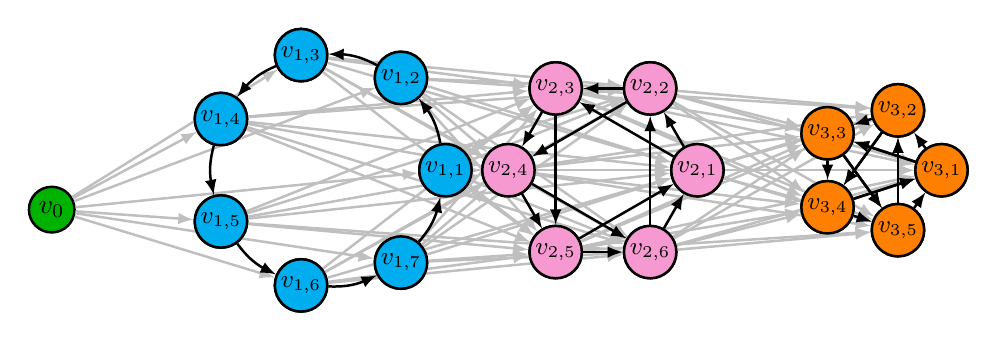
\begin{tikzpicture}[>=latex, line width=0.9pt]
			
			% --- 2. Nodes (Main Layer) ---
			% R0 Parent
			\node[fill=green!70!black,draw, circle, inner sep=2pt] (v0) at (0, -0.5) {\(v_0\)};
			
			% R1 Cycle Nodes
			\def\n{7} \def\radius{1.5} \def\centerx{3.5}
			\foreach \i in {1,...,\n} {
				\node[fill=cyan, draw, circle, inner sep=1.2pt] (v1\i) at ({\centerx + \radius*cos(360/\n*(\i-1))}, {\radius*sin(360/\n*(\i-1))}) {\small \(v_{1,\i}\)};
			}
			
			% R2 Cycle Nodes
			\def\m{6} \def\rradius{1.2}
			\foreach \i in {1,...,\m} {
				\node[fill=magenta!40,draw, circle, inner sep=1.2pt] (v2\i) at ({2*\centerx + \rradius*cos(360/\m*(\i-1))}, {\rradius*sin(360/\m*(\i-1))}) {\small \(v_{2,\i}\)};
			}
			
			% R3 Cycle Nodes
			\def\p{5} \def\rrradius{0.8}
			\foreach \i in {1,...,\p} {
				\node[fill=orange,draw, circle, inner sep=1.2pt] (v3\i) at ({3*\centerx + \rrradius*cos(360/\p*(\i-1))}, {\rrradius*sin(360/\p*(\i-1))}) {\small \(v_{2,\i}\)};
			}
			
			% --- 3. Arcs (Background Layer) ---
			% Arcs from R0 to R1
			\foreach \i in {1,...,\n} {
				\draw[lightgray,->] (v0) -- (v1\i);
			}
			
			% Arcs from R1 to R2
			\foreach \i in {1,...,\n}{
				\foreach \j in {1,...,\m} {
					\draw[lightgray,->] (v1\i) -- (v2\j);
				}
			}
			
			% Arcs from R2 to R3
			\foreach \i in {1,...,\m}{
				\foreach \j in {1,...,\p} {
					\draw[lightgray,->] (v2\i) -- (v3\j);
				}
			}
			
			% R1 Interior Arcs
			\foreach \i [evaluate=\i as \next using {int(mod(\i,\n)+1)}] in {1,...,\n} {
				\draw[->, bend right=15] (v1\i) to (v1\next);
			}
			
			% R2 Interior Arcs
			\foreach \i [evaluate=\i as \next using {int(mod(\i,\m)+1)},
			evaluate=\i as \afternext using {int(mod(\i+1,\m)+1)}] in {1,...,\m} {
				\draw[->] (v2\i) to (v2\next);
				\draw[->] (v2\i) to (v2\afternext);
			}
			
			% R3 Interior Arcs
			\foreach \i [evaluate=\i as \next using {int(mod(\i,\p)+1)},
			evaluate=\i as \afternext using {int(mod(\i+1,\p)+1)},
			evaluate=\i as \afterafternext using {int(mod(\i+1,\p)+1)}] in {1,...,\p} {
				\draw[->] (v3\i) to (v3\next);
				\draw[->] (v3\i) to (v3\afternext);
				\draw[->] (v3\i) to (v3\afterafternext);
			}
			
			% R1 Cycle Nodes
			\def\n{7} \def\radius{1.5} \def\centerx{3.5}
			\foreach \i in {1,...,\n} {
				\node[fill=cyan, draw, circle, inner sep=1.2pt] (v1\i) at ({\centerx + \radius*cos(360/\n*(\i-1))}, {\radius*sin(360/\n*(\i-1))}) {\small \(v_{1,\i}\)};
			}
			
			% R2 Cycle Nodes
			\def\m{6} \def\rradius{1.2}
			\foreach \i in {1,...,\m} {
				\node[fill=magenta!40,draw, circle, inner sep=1.2pt] (v2\i) at ({2*\centerx + \rradius*cos(360/\m*(\i-1))}, {\rradius*sin(360/\m*(\i-1))}) {\small \(v_{2,\i}\)};
			}
			
			% R3 Cycle Nodes
			\def\p{5} \def\rrradius{0.8}
			\foreach \i in {1,...,\p} {
				\node[fill=orange,draw, circle, inner sep=1.2pt] (v3\i) at ({3*\centerx + \rrradius*cos(360/\p*(\i-1))}, {\rrradius*sin(360/\p*(\i-1))}) {\small \(v_{3,\i}\)};
			}		
		\end{tikzpicture}
		\caption{\textit{BFS \& Lex Graph in an MCE. The minimum out-degree is 7. Nodes are arranged according to their BFS layers. Each node within these layers is assigned a distinguishing distance \& lexicographic ID.} } \label{earlyssnc}
	\end{figure}
	
	
	\vspace{2.8ex}
	%	\begin{minipage}{0.8\textwidth}
		\noindent\hrulefill
		\begin{example}
			
			In this section, we construct an example demonstrating how non-Seymour vertices can be embedded within a MCE environment of minimum out-degree $\delta^+(G) = 7$. Let $v_0$ be a vertex with minimum out-degree, and let $R_k = \{v \in V(G) \mid \text{dist}(v_0, v) = k\}$ denote the $k$-th out-neighborhood of $v_0$. We initialize the construction by setting $R_0 = \{v_0\}$. Since $\delta^+(G) = 7$, $|R_1| = 7$. For $v_0$ to be a non-Seymour vertex, its second out-neighborhood must satisfy $|R_2| < |R_1|$, implying $|R_2| \le 6$.
			
			Let $G[R_1]$ be te subgraph induced bt $R_1$ and let $G[R_2]$ be the subgraph induced by $R_2$. The nodes in $R_1$ are first neighbors of $v_0$ and the nodes in $R_2$ are the second neighbors. By the pigeonhole principle, to make $v_0$ a non-Seymour vertex, we need to establish that $|R_2| < |R_1| = \delta$. This gives a maximum size of $\delta - 1$ on $R_2$, forcing every node in $R_1$ to have at least one interior neighbor. Lemma \ref{extraArcs} shows that no node in $R_1$ can have a higher more than one same level cross arc, forcing these nodes to be regular at distance 1.
			
			We next examine the vertices in $R_2$, which similarly must satisfy $\delta^+(G) = 7$. Again, the pigeonhole principle applies here to make the nodes in $R_1$ non-Seymour. As $|R_2| = \delta - 1$ has already had its capacity limited, there are even fewer holes for the pigeons to land in here. Consequently, we see that to make nodes in $R_1$ non-Seymour, these nodes must each connect to two arcs in $R_2$. Corollary \ref{noDLBack} shows that back arcs are not possible in this case.
			If a parent vertex $u_1 \in R_1$ of $u_2$ satisfies $|R_2| \le |R_3|$, then $u_1$'s forward property is Seymour. Similarly, because it has already been shown that $u_1$ has a degree $\le 6$ in $R_1$ irs local property is Seymour as well.. This implies that $u_1$ is a Seymour vertex. Thus, we must have $d^+_{G[R_2]}(u) \ge 2$ for all $u \in R_2$.
			
			To summarize, the cardinality of the rooted neighborhoods required to pack these non-Seymour vertices is given by:
			
			\begin{itemize}
				\item $|R_0| = |\{v_0\}| = 1$.
				\item $|R_1| = |\{v \in V(G) \mid \text{dist}(v_0, v) = 1\}| = 7$.
				\item $|R_2| = |\{v \in V(G) \mid \text{dist}(v_0, v) = 2\}| = 6$.
				\item $|R_3| = |\{v \in V(G) \mid \text{dist}(v_0, v) = 3\}| = 5$.
			\end{itemize}
			
			Finally, consider the vertices in $R_3$. To prevent their respective parent vertices from becoming Seymour vertices, the vertices in $R_3$ must maintain an internal induced out-degree of $d^+_{G[R_3]}(v) \ge 3$. This configuration requires at least $3 \times |R_3| = 15$ arcs within $G[R_3]$. However, a simple graph on 5 vertices can sustain at most $\binom{5}{2} = 10$ arcs. These nodes will be unable to meet their necessary out-degree requirements through local $R_3$ cycles. Thus either back arcs (to nodes with more second neighbors) are necessary, or an equal or larger $R_4$. Either of these conditions creates Seymour vertices.
			
			By this contradiction, the vertices in $R_3$ are guaranteed to be Seymour vertices.
		\end{example}
		\noindent\hrulefill
		%	\end{minipage}
	\vspace{2.8ex}
	
	As the number of second neighbors is iteratively reduced, nodes must compensate by connecting to more of their own siblings. This allows their parents to become non-Seymour nodes. The out-neighbors must form forward facing transitive triangles. These triangles must repeatedly interlock to form cycles to reduce the parent's second neighborhood.
	
	
	\begin{theorem}[Graph Level Order Representation of Oriented Graphs]\label{gloverrep}
		Every oriented graph $G = (V,E)$ can be represented by a Graph Level Order. \end{theorem}
	\begin{proof}
		We present an algorithm for this procedure.
		\begin{enumerate}
			\item Select a minimum out-degree root
			\item Define rooted neighborhoods. For each $i \ge 1$, define $$ R_i = \{ u_i \in V : \text{dist}(v_0, u_i) = i \}, $$
			\item Total order within neighborhoods. Within each $R_i$, impose a consistent total order on vertices (e.g., lexicographic or another ordering).
			\item Parent–child relations. For $u_i \in R_i$ and $v_{i+1} \in R_{i+1}$, if $u_i \to v_{i+1} \in E$, declare $u_i$ a parent and $v_{i+1}$ a child. This defines interior and exterior neighbors $u_i \to v_{i+1}$: $$ \text{int}(u_i,v_{i+1}) = N^+(u_i) \cap N^+(v_{i+1}) \cap R_{i+1}, \quad \text{ext}(u_i,v_{i+1}) = N^{++}(u_i) \cap N^+(v_{i+1}) \cap R_{i+2}. $$
		\end{enumerate}
		By construction, every out-neighbor of $v$ in $R_{i+1} \cup R_{i+2}$ is either interior or exterior relative to its parent $u$.
		
		\medskip Thus, $G$ is fully described by the rooted neighborhoods $R_0, \dots, R_k$, the parent–child relations, and the interior/exterior neighbor sets. This satisfies all the properties required for a Graph Level Order representation.
	\end{proof}
	
	Because of this universal representation of graphs, when we speak of oriented graphs we are always talking of a Graph Level Order environment.
						
	\subsection{Using Graph Level Order}
	
	With the Graph Level Order vocabulary established, these definitions now must connect to the mathematical foundation. Interior neighbors relate to the first neighbors of a parent. Exterior neighbors relate to the second neighbors. In an MCE environment, Theorem \ref{lbl} (Load Balance) shows the only purpose of these interior neighbors is to be forward-facing transitive triangles that reduce the parent’s second neighborhood.
			
			%	An edge $e$ is \textbf{unnecessary} to the MCE $G$ if replacing $e$ with an forward arc $e'$ in the MCE results in a graph that preserves the non-Seymour status of all vertices ($|N^{++}_{G'}(v)| < |N^{+}_{G'}(v)|$ for every $v \in V$).
			
				\begin{theorem}[Rooted Neighborhood Equivalence Relation]\label{nbhequiv}
		Let $G$ be a Minimum Counterexample (MCE). Every vertex within a rooted neighborhood $R_k$ is indistinguishable under the rooted degree-preserving mapping $\sim$. The resulting quotient graph $G/\sim$ is a well-defined hyper-node graph that preserves the out-degree and non-Seymour status of $G$.
	\end{theorem}
	\begin{proof}
		Let $v_k, w_k \in R_k$. By Theorem \ref{bfslex}, these nodes have identical parents because they lie at the same distance. Lemma \ref{nodepartition} (Degree Partition) implies that the degrees of $v_k$ and $w_k$ can be partitioned into interior and exterior components. Theorem \ref{lbl} (Load Balance) establishes that both nodes possess identical interior degrees of $k$. 
		
		Furthermore, since back arcs are excluded by Corollaries \ref{noDLBack} (No Disconnected Layer Back Arcs) and \ref{noCLBack} (No Connected Layer Back Arcs), they possess identical exterior neighbors. In addition, by Theorem \ref{lbl} (Load Balance), all interior arcs of $v_k$ and $w_k$ must induce forward-facing transitive triangles. Because these are the unique load-balancing triangles permitted by Theorem \ref{lbt} (Load-Balancing Triangles), the rooted induced subgraphs $G[R(v_k)]$ and $G[R(w_k)]$ are isomorphic under a neighborhood-preserving mapping fixing the root. 
		
		Since this structural equivalence holds for all pairs in $R_k$, the set $R_k$ constitutes an equivalence class under a rooted degree-preserving mapping. Collapsing these classes yields a well-defined quotient graph $G/\sim$ that preserves out-degrees and preserves the non-Seymour counterexample property.
	\end{proof}
	
	The rooted neighborhood equivalence relation structure can be seen in Figure \ref{earlyssnc}. As shown in Section \ref{glover}, every node in the graph has an out-degree of 7. By neighborhood, all nodes at distance one have interior out-degree of one. All nodes at distance two have an interior out-degree of two. Nodes having the same distance from the root, interior and exterior exterior neighbor set, making them rooted degree equivalent.
	
	\begin{remark}[The Equivalence Relation is a Hyper-Graph, Not a Line Graph]
		The rooted degree equivalence $\sim_k$ partitions $V$ into equivalence classes $R_0, R_1, \ldots, R_m$. Each class $R_k$ is collapsed to a single hyper-node forms a directed path on $m+1$ hyper-nodes. This is a 
		property of the \emph{quotient hyper-graph}, not of $G$ itself. 
		The original graph $G$ is not a line graph or a path --- it retains its full vertex set, arc set, and internal cycle structure within each layer $R_k$.
	\end{remark}
	
	
	\begin{lemma}[GLO Bridge] Let $G$ be an MCE with GLO decomposition $R_0, R_1, ..., R_m$. ,. For any parent $p \in R_{k-1}$ \label{bridge}
		\[N^+(p) = R_k,\] \[N^{++}(p) = R_{k+1}\]
		
		Consequently, the SSNC condition $|N^{++}(p)| < |N^+{p}|$ is equivalent to $|R_{k+1}| < |R_k|$. 
	\end{lemma}
	\begin{proof}
		By Theorem\ref{lbl}, every parent $p \in R_{k-1}$ has forward degree $\delta - (k-1) = \delta - k +1 = |R_K|$. Since no back arcs exist (\ref{noDLBack} and \ref{noCLBack}, all $\delta - k + 1$ forward arcs of $p$ land in $R_k$, which has exactly $\delta - k + 1$ vertices. Therefore $N^+_{fwd}(p) = R_k$, giving $N^+(p) = R_k$. 
		
		Every vertex $v_k \in R_k = N^+(p)$ has forward arcs into $R_{k+1}$. By Theorem \ref{lbl}, these forward neighborhoods are uniform and together cover $R_{k+1}$ completely. Therefore $N^{++}(p) = R_{k+1}$. 
		
		It follows that $|N^+(p)| = {R_k}$ and $|N^{++}(p)| = |R_{k+1}|$. so $|N^{++}(p)| < N^+(p)|$ if and only if $|R_{k+1}| < |R_{k}|$. 
	\end{proof}
	
	\begin{corollary}[Hierholzer's Algorithm]\label{ilb}
		Let $G=(V,E)$ be an MCE to the SSNC with root $v_0$ and let $R_k$ be a rooted neighborhood at distance $k$ from $v_0$. Because every node has interior degree of $k$ in $R_k$ Hierholzer's Algorithm will find at least $k$ disjoint cycles in $R_k$.
	\end{corollary}
	
	\begin{figure}
		\centering
		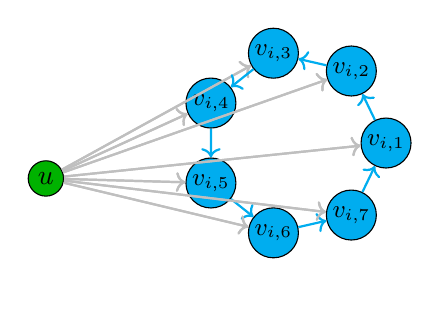
\begin{tikzpicture}[scale=0.9]
			% Parent Node (R_0)
			\node[fill=green!70!black, draw, circle, inner sep=2pt] (v0) at (0, -0.5) {\(u\)};
			
			% Parameters for the cycle
			\def\n{7}
			\def\radius{1.3}
			\def\centerx{3.5}
			
			% Draw the Cycle of Neighbors (v_i) in R_1
			\foreach \i in {1,...,\n} {
				\node[fill=cyan, draw, circle, inner sep=1.2pt] (v1\i) at ({\centerx + \radius*cos(360/\n*(\i-1))}, {\radius*sin(360/\n*(\i-1))}) {\small \(v_{i,\i}\)};
			}
			
			% Build the regular cycle (Slides 1-7)
			\foreach \start/\target in {4/5, 5/6, 6/7, 7/1, 1/2, 2/3, 3/4}
			{
				\draw [lightgray, ->, thick] (v0) -- (v1\start);
				\draw [lightgray, ->, thick] (v0) -- (v1\target);
				\draw [cyan, ->, thick] (v1\start) -- (v1\target);
			}
			
			% The "Stray" Forbidden Arc (Slide 8)
			Using red and dashed to signify "This is banned"
			%		\draw<8> [red, dashed, thick, ->, bend left=20] (v15) to node[auto] {\small %\textbf{Double-Covered}} (v17);
			
			% Labeling
			\node[anchor=north] at (\centerx, -2) {
				% \only<1-7>{Constructing the MCE-mandated regular cycle...}
				% \only<8>{By minimality, extra interior arcs (like $v_{1,5} \to v_{1,7}$) are infeasible.}
			};
		\end{tikzpicture}
		\caption{ \textit { \textbf{Set cover implies a cycle}. Nodes have out-degree = 1 in $N^+(u)$. This implies the existence of at least one cycle in $N^+(u)$, allowing for a reduction in the size of $N^{++}(u)$.  }}
	\end{figure}
		
	\begin{figure}
		\centering
		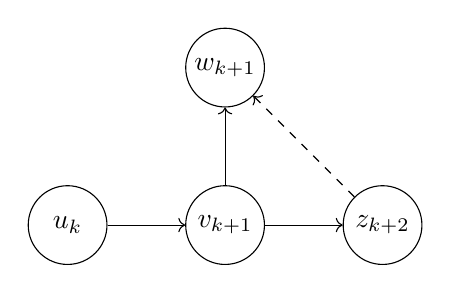
\begin{tikzpicture}[
			every edge/.style = {draw,->},
			Vertex/.style = {circle, draw, minimum size=1cm, inner sep=0pt},
			]
			% Define the nodes
			\node[Vertex] (u_k) at (0, 0) {\(u_k\)};
			\node[Vertex] (v_{k+1}) at (2,0) {\(v_{k+1}\)};
			\node[Vertex] (w_{k+1}) at (2,2) {\(w_{k+1}\)};
			\node[Vertex] (z_{k+2}) at (4,0) {\(z_{k+2}\)};
			
			% Draw directed edges between nodes
			\draw[->] (u_k) -- (v_{k+1});
			\draw[->] (v_{k+1}) -- (z_{k+2});
			\draw[->] (v_{k+1}) -- (w_{k+1});
			\draw[->, dashed] (z_{k+2}) -- (w_{k+1});
			
		\end{tikzpicture}
		\caption{\textit{\textbf{False Flag problem of back arcs}. Assuming that $z_{k+2} \to w_{k+1}$ is the first back arc, $w_{k+1}$ must map to a new exterior neighbor. This will make $u_k$ a Seymour vertex.} }\label{backexwk}
	\end{figure}
	
	The rooted structure of the Graph Level Order is an important characteristic. Consider Example \ref{backexwk}. At first glance, the back arc $z_{k+2} \to w_{k+1}$ may seem to violate the principles of the Graph Level Order. However, this does not take into account their respective distances from the root node. Assuming this is the first back arc, what we can show is that this back arc cannot exist.
	
	Let $u_k$ be at distance $k$. Then $v_{k+1}$ and $w_{k+1}$ are at distance $k+1$ and $z_{k+2}$ is at distance $k+2$. The nodes $v_{k+1}$ interior degree must be $k+1$, implying they have $\delta-k-2$ exterior neighbors. One of $v_{k+1}$'s exterior neighbors is $z_{k+2}$, but $w_{k+1}$ cannot relate to $z_{k+2}$ by definition of an oriented graph. This node $w_{k+1}$ must still have $\delta-k-2$ exterior neighbors. So $w_{k+1}$ must relate to a new node $y_{k+2}$. This means that $u_k$'s second neighborhood did not decrease by one as the Load Balance Theorem \ref{lbl} says it must by the cycles in its first neighborhood. Thus, $u_k$ will be is a Seymour vertex.
	
	By definition, an MCE is always on the edge of collapse. Maximizing the number of non-Seymour nodes formalizes this fragility. Although it is invoked as a contradictory hypothesis, the argument is inherently constructive. The graph was set up based on distance. Set-theoretic, ancestral neighborhoods were constructed to resolve past obstructions. This is explicitly explaining why these things happened.
	
	Let $G \in \mathcal{O}$ be an oriented graph represented by a Graph Level Order. Define $v_k \sim w_k$ for two vertices $v_k, w_k \in R_k$ if there exists a rooted degree preserving mapping on $G$ fixing $v_0$ and preserving rooted neighborhoods $R_i$ such that $v_k \mapsto w_k$
	
	\subsection{Power of the Data Structure}\label{power}
	This would be a futile attempt at proving the SSNC if we could not manage the complications mentioned in previous papers. First are transitive triangles, where Brantner et al. \cite{BBKS} showed that oriented graphs without transitive triangles contain a Seymour vertex, the MDN.
	
	\begin{theorem}[Load-Balancing Triangles]\label{lbt}The only possible transitive triangles in an MCE are load-balancing triangles.\end{theorem}
	\begin{proof}
		We classify all transitive triangles by examining the first two arcs and determine whether a valid third arc can close the triangle.
		
		A triangle has three arcs, so there are $2^3 = 8$ possible combinations of arc types. We enumerate these cases in Table \ref{transtricases}:
		\begin{table}[h!]
			\centering
			\begin{tabular}{|c|c|c|c|} \hline Case
				& Labels & Triangle Possible? & Reason
				\\ \hline
				1 & 3I & Yes & (all Intra-layer)\\
				\hline
				2, 4 & 1B2I / 1F2I & No & Symmetric Arcs \\
				\hline
				3 & 2B1I & Yes & $x,y \in R_i$, $z \in R_{i+1},x \to y,z \to x,z \to y$\\
				\hline
				5 & 1F1B1I & Yes &$x, y \in R_i, z\in R_{i+1}, x \to y,x \to z,z \to y$. \\
				\hline
				6 & 1F2B & Yes & $x \in R_i ,y \in R_{i+1},z \in R_{i+2},x \to y$,$z \to x$,$z \to y$. \\
				\hline
				7 & 2F1I & Yes &$x\in R_i,y,z \in R_{i+1},x \to y, x \to z, y \to z$. \\
				\hline
				8 & 2F1B & No & \makecell{cannot form a closed transitive triangle.} \\
				\hline
			\end{tabular} \caption{Eight possible configurations of transitive triangles in a Graph Level Order.}
			\label{transtricases}
		\end{table}
		
		From these 8 possible cases, three are excluded immediately because of impossibility (Cases 2, 4, 8). Theorem \ref{red} (Reduction) says that back arcs are unnecessary in an MCE (Cases 3, 5, and 6).
		
		The remaining triangles are the following: Case 1: $x \to y \to z \to x$, all in $R_i$, and the Load-Balancing Triangle (Case 7). A triangle from Case 1 is not a load-balancing triangle, so it contains an extra interior arc. By Theorem \ref{lbl} (Load Balance) $G$ cannot be an MCE.
	\end{proof}
			
	\begin{theorem}[Resolution of Seymour Diamonds]\label{smdiam}
		Let $G \in \mathcal{O}$ be a Graph Level Order containing a Seymour diamond. Then the ambiguity is resolved via exterior neighbors. \end{theorem}
	
	\begin{proof}
		Assume $G$ has a Seymour diamond $u_i, v_{i+1}, w_{i+1},y_{i+2}$.
		By theorem \ref{red} (Reduction),
		$$N^{++}(u_i) = \bigcup_{v_{i+1} \in {N^+(u_i)}} \text{ext}(u_i, v_{i+1}).$$
		
		The exterior neighbors are sets, so any node reached by multiple length-2 paths is counted only once in $N^{++}(u_i)$.
		This eliminates double-counting for the node $u_i$.
	\end{proof}
			
The two main hindrances of this conjecture have been shown that they are not roadblocks. The data structure used throughout this paper has been defined. This data structure provides an understanding of interior and exterior arcs, and guides the search for a counterexample. It also provides understanding of non-Seymour nodes and guides the nodes in this proof process.

\section{Main Theorem} \label{main}

\begin{example}
	\begin{table}[h!]
		\centering
		\begin{tabular}{|c|c|c|}
			\hline
			\textbf{Rooted Neighborhood} & \textbf{Nodes} & \textbf{Size} \\
			\hline
			$R_0$ & 0 & 1 \\
			$R_1$ & 1, 2, 3 & 3 \\
			$R_2$ & 4, 5 & 2 \\
			\hline
		\end{tabular}
		\caption{\textit{A look at Example minimum out-degree 3 example through the lens of rooted neighborhoods and their sizes}} \label{exdegdoub2}
	\end{table}
\end{example}

We begin this section by contrasting two examples. Tables \ref{exdegdoub2} and \ref{exdegdoub12} give two different reasons for the emergence of a Seymour vertex. In Table \ref{exdegdoub2}, the presence of an oriented graph of size two implies that both those nodes cannot have an out-degree of 1. That would violate the oriented graph property. Hence, a node in $R_2$ needs to send at least 3 nodes to $R_3$ forcing a node in $R_1$ to be a Seymour vertex.

Conversely, Table \ref{exdegdoub12} because of the neighborhood density of $R_3$. There are 5 nodes in $R_3$ at distance 3 from the root. Theorem \ref{lbl} (Load Balance) requires each node in $R_3$ to have an interior degree of $3$. This requires 15 arcs. This is impossible, as a 5-node oriented graph can have only 10 arcs by the binomial theorem. This will force a Seymour vertex.

\begin{example}
	\begin{table}[h!]
		\centering
		\begin{tabular}{|c|c|c|}
			\hline
			\textbf{Rooted Neighborhood} & \textbf{Nodes} & \textbf{Size} \\
			\hline
			$R_0$ & 0 & 1 \\
			$R_1$ & 1, 2, 3, 4, 5, 6, 7 & 7 \\
			$R_2$ & 8, 9, 10, 11, 12, 13 & 6 \\
			$R_3$ & 14, 15, 16, 17, 18 & 5 \\
			\hline
		\end{tabular}
		\caption{\textit{Minimum out-degree 7 example through the lens of rooted neighborhoods}} \label{exdegdoub12}
	\end{table}
\end{example}

\pgfplotsset{compat=1.18}
\begin{figure}
	\centering
	\begin{tikzpicture}[scale=0.7]
		\begin{axis}[
			width=11cm,
			height=7cm,
			xlabel={Minimum out-degree $\delta$},
			ylabel={Termination depth},
			xmin=2.5, xmax=14.5,
			ymin=0.5, ymax=6,
			xtick={3,4,5,6,7,8,9,10,11,12,13,14},
			ytick={1,2,3,4,5},
			grid=both,
			grid style={dashed, gray!30},
			legend style={at={(0.02,0.98)},anchor=north west}
			]
			
			% Scatter points
			
			\addplot[
			only marks,
			mark=*,
			mark size=2pt
			] coordinates {
				(3,2)
				(4,2)
				(5,2)
				(6,3)
				(7,3)
				(8,3)
				(9,4)
				(10,4)
				(11,4)
				(12,5)
				(13,5)
				(14,5)
			};
			
			\addlegendentry{Observed termination depth}
			
			% Linear interpolation
			
			\addplot[
			thick,
			blue,
			domain=3:14
			] {(x-1)/3 + 1};
			
			\addlegendentry{Linear trend $y = \delta/3 + 1$}\begin{tikzpicture}[
				every node/.style={draw, rectangle, rounded corners, minimum height=7mm},
				arrow/.style={->, thick}
				]
			\end{tikzpicture}
		\end{axis}
	\end{tikzpicture}
	\caption{\textit{The scatter points represent the last feasible rooted neighborhood before non-decreasing is forced. The linear trend illustrates the bound predicted by Corollary~\ref{smfmla}, showing termination at approximately $\lceil\delta/3\rceil$.}}
	
\end{figure}\label{scattplt}

Example \ref{scattplt} shows the feasibility of rooted neighborhoods with minimum out-degree values $\delta$ ranging from 3 to 14. A clear pattern is evident, as shown by the trend line. Regardless of $\delta$, a Seymour vertex is always found at $\lfloor \frac{\delta}{3} \rfloor+1$. This is discussed further in Theorem \ref{smfmla} (Last Rooted Neighborhood).

\begin{figure}
	\centering
	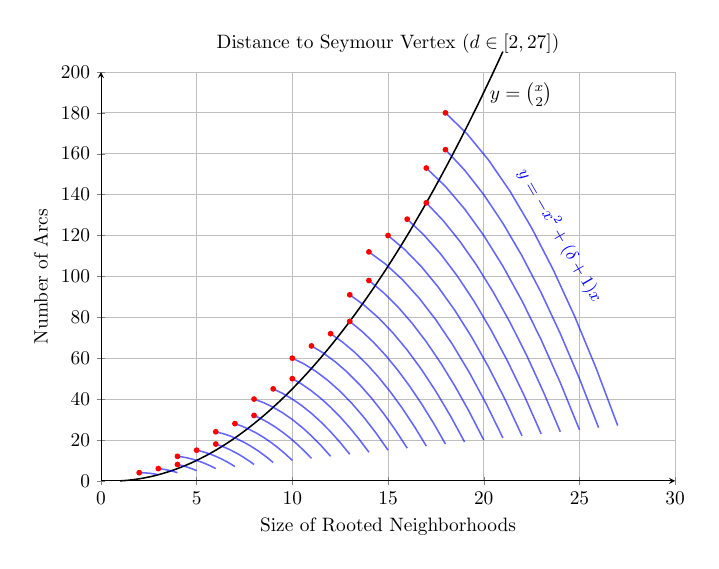
\begin{tikzpicture}[scale=0.7]
		\begin{axis}[
			width=12cm, height=9cm,
			axis lines=left,
			grid=both,
			xmin=0, xmax=30,
			ymin=0, ymax=200,
			xlabel={Size of Rooted Neighborhoods},
			ylabel={Number of Arcs},
			title={Distance to Seymour Vertex ($d \in [2, 27]$)},
			clip=false
			]
			
			% 1. Boundary: y = x(x-1)/2
			\addplot[thick, black, domain=1:21, samples=100] {x*(x-1)/2}
			node[pos=0.9, right] {$y = \binom{x}{2}$};
			
			% 2. Automated Path Generator using \pgfplotsinvokeforeach
			% Note: Use #1 instead of \d inside this command
			\pgfplotsinvokeforeach{3,4,...,27}{
				\addplot[blue, thick, opacity=0.6, domain=0:{floor(#1/3)}, samples=9]
				({ #1 - x }, { (#1 - x) * (x + 1) });
				% y = -x^2 + (d+1)x
				% Draw the red dot at the Sink
				\fill[red] (axis cs:{ #1 - floor(#1/3) }, { (#1 - floor(#1/3)) * (floor(#1/3) + 1) }) circle (1.5pt);
			}
			\node[blue, font=\small, rotate=-60] at (axis cs:24,120) {$y = -x^2 + (\delta+1)x$};
		\end{axis}
	\end{tikzpicture}
	\caption{\textit{\textbf{Emergence of a maximally dense, rooted neighborhood}. Blue state-transition paths show the contraction of rooted neighborhood size (supply) and quadratic growth in interior arc requirements (demand). These are bounded above by $y=\binom{x}{2}$. Their intersection causes a terminal sink that corresponds to the last dense, rooted neighborhood with multiple Seymour vertices. Each of these blue lines is plotted along the quadratic arc of $y = -x^2 + (\delta+1) \cdot x$. }}
	\label{lastneightbl}
\end{figure}

Figure \ref{lastneightbl} illustrates the fundamental breakdown that occurs when the model's supply and demand requirements clash within these rooted neighborhoods. Vertex capacity decreases linearly. The interior arc requirements grow quadratically. This is modeled by the equation $y = -x^2 + (\delta + 1)\cdot x$.

The concavity of these paths reflects the accelerating neighborhood density required to maintain a decreasing sequence of neighborhoods. The $(\delta+1) \cdot x$ term is the ideal arc count. It is the Load Balance Theorem \ref{lbl} showing the balance between interior and exterior neighbors. The $-x^2$ is the compression penalty issued by the non-Seymour nodes. The resulting equation $(\delta+1)x - x^2$ is the actual internal neighborhood density. The variable $x$ is a double metric, defining both the distance from the root and the number of arcs required per node at that distance.

\begin{theorem}[Last Rooted Neighborhood] \label{smfmla}
	Let $G$ be an oriented graph with minimum out-degree $\delta \ge 3$. Let $\mathcal{R} = \{R_0, R_1, \dots, R_k\}$ be the rooted neighborhoods of $V$ originating at a root $v_0$ of minimum out-degree.
	
	If every $u \in G$ is non-Seymour, then:
	\begin{enumerate}
		\item The maximum number of rooted neighborhoods is bounded by $k = \lceil \frac{\delta}{3} \rceil$.
		\item The cardinality of the terminal level set is $|R_k| = \delta - k + 1$.
		\item Every node in $R_{k-1}$ belongs to at least $k-1$ disjoint cycles.
	\end{enumerate}
\end{theorem}
\begin{proof}
	Fix $i \ge 1$ and consider the rooted neighborhood $R_i$. By the Load Balance Theorem \ref{lbl}, every node in $R_i$ must have an interior degree of exactly $i$. The Iterative Load-Balance Corollary \ref{ilb} converts each node's interior degrees into transitive triangles, yielding a required set of disjoint interior arcs of size:
	\[ |R_i| \cdot i \tag{1} \]
	
	As an oriented graph, the number of interior arcs in $R_i$ is bounded above by the maximum number of oriented off-diagonal pairs among vertices in $R_i$:
	\[ |E(R_i)| \le \binom{|R_i|}{2} = \frac{|R_i|(|R_i| - 1)}{2} \tag{2} \]
	
	Combining (1) and (2) gives the feasibility condition:
	\[ |R_i| \cdot i \le \frac{|R_i|(|R_i| - 1)}{2} \quad \implies \quad 2i \le |R_i| - 1 \quad \implies \quad |R_i| \ge 2i + 1. \tag{3} \]
	
	Next, by Corollary \ref{nbhsizefmla} (Formula for Rooted Neighborhood Size), the assumption that all nodes are non-Seymour enforces a global contraction of neighborhoods across levels:
	\[ |R_i| = \delta - (i - 1) = \delta - i + 1. \tag{4} \]
	
	Substituting (4) into the lower bound from (3):
	\[ \delta - i + 1 \ge 2i + 1 \quad \implies \quad \delta \ge 3i \quad \implies \quad i \le \frac{\delta}{3}. \tag{5} \]
	
	Thus, for any rooted neighborhood $R_i$ to exist without forcing Seymour vertices, the depth index $i$ cannot exceed $\lceil \frac{\delta}{3} \rceil$. 
	
	When $i$ exceeds $\frac{\delta}{3}$, inequality (5) fails: the required number of interior arcs strictly exceeds the capacity that $R_i$ can support. This deficit forces additional exterior arcs to be redirected inward. By the Load Balance Theorem \ref{lbl}, this redirection produces supplementary transitive triangles, which guarantees the existence of a Seymour vertex. Therefore, the rooted neighborhoods cannot extend beyond $k = \lceil \frac{\delta}{3} \rceil$, establishing both the level bound and the terminal cardinality $|R_k| = \delta - k + 1$. Part (3) follows directly from the guaranteed accumulation of $k-1$ disjoint cycles required to sustain the interior degree constraint at depth $k-1$.
\end{proof}

\begin{figure}
	\centering
	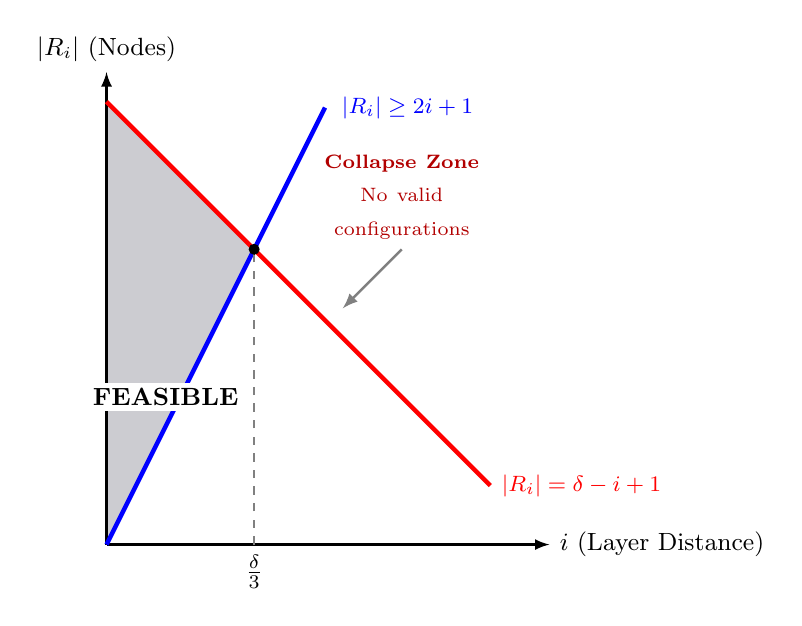
\begin{tikzpicture}[>=latex, line width=0.9pt, scale=0.75]
		% Variables
		\def\deltaVal{9}
		\def\intersectX{3} % Calculated: 2i+1 = 9-i+1 => 3i = 9 => i=3
		\def\intersectY{7}
		
		% Shaded feasible region with pattern
		\fill[blue!10!black!20] (0.5,2) -- plot[domain=0.5:\intersectX] (\x, {2*\x + 1})
		-- plot[domain=\intersectX:0.5] (\x, {\deltaVal - \x + 1}) -- cycle;
		
		% Axes
		\draw[->, thick] (0.5,2) -- (0.5,10) node[above] {\small $|R_i|$ (Nodes)};
		\draw[->, thick] (0.5,2) -- (8.0,2) node[right] {\small $i$ (Layer Distance)};
		
		% Constraint 1: Supply
		\draw[blue, ultra thick, domain=0.5:4.2] plot (\x, {2*\x + 1})
		node[right, xshift=2pt] {\footnotesize $|R_i| \ge 2i+1$};
		
		% Constraint 2: Demand
		\draw[red, ultra thick, domain=0.5:7] plot (\x, {\deltaVal - \x + 1})
		node[right] {\footnotesize $|R_i| = \delta-i+1$};
		
		% Intersection & Collapse marker
		\draw[dashed, gray] (\intersectX, 2) -- (\intersectX, \intersectY);
		\filldraw[black] (\intersectX, \intersectY) circle (2pt);
		
		% Labels
		\node[below] at (\intersectX, 2) {$\frac{\delta}{3}$};
		\node[fill=white, inner sep=2pt] at (1.5, 4.5) {\small \textbf{FEASIBLE}};
		
		% Annotation for the Collapse
		\draw[<-, gray] (4.5, 6) -- (5.5, 7) node[above, text width=2cm, align=center]
		{\scriptsize \color{red!70!black} \textbf{Collapse Zone} \\ No valid configurations};
		
	\end{tikzpicture}
	\caption{\textit{\textbf{Intersection of Supply and Demand.} Supply is the number of nodes necessary for a MCE, bounded by the binomial theorem ($|R_i| \geq 2\cdot i + 1$). Demand is controlled by the decreasing size of the rooted neighborhoods. Beyond the threshold of $i = \delta/3$, there are no possibilities to support the interior cycles necessary, resulting in a collapse.
	}}
\end{figure}

Any directed graph $G \in \mathcal{O}$ in an MCE with more than three nodes will eventually have a last rooted neighborhood at distance $\lceil \delta / 3 \rceil$ by \ref{smfmla}. The size of this neighborhood will be $\lceil 2 \dot \delta / 3 \rceil$. This is an integer greater than 1 as long as $\delta > 1.5$, which must be true for there to be cycles to be present in $G$.

\begin{corollary}[Multiple Seymour Vertices] \label{multiDDNodes}
	Let $G \in \mathcal{O}$ be an oriented graph with minimum out-degree $\delta$, and let $R_i$ be the last, most dense rooted neighborhood. Then every node in $R_i$ is a Seymour vertex.
\end{corollary}

\subsection{Algorithm \& Complexity Theory}

\begin{theorem}[Algorithm Complexity] \label{complx}
	Let $G$ be an oriented graph. The Graph Level Order algorithm runs in $$O(|V| + |E|),$$ where $|V|$ is the number of vertices and $|E|$ is the number of edges in $G$.
\end{theorem}
The proof follows the implementation of the BFS algorithm through the neighborhoods. Each node is visited only one time, giving it an $O(|V| + |E|)$ time.

The algorithm can find a Seymour vertex in linear time. Moreover, it will work for any oriented graph. The analysis shows that it will not be a problem on larger graphs.

\section{Conclusion}

This work approached the SSNC through a minimum counterexample angle. Naturally, that led to layered embeddings of oriented graphs. By starting from a minimum out-degree node, the well ordering that was established gave the minimum counterexample its power.

The key insight is that BFS is not simply a traversal algorithm. Along with lexicographic ordering, this algorithm can impose a well-ordering on a graph. By connecting the neighborhoods to BFS layers, the structure of Seymour vertices became dependent on cycle packing.

This work also introduces techniques of partitioning and the dual metrics of degree and distance. These methods may apply beyond the SSNC, especially to problems in graph theory that invite constructive, algorithmic approaches rather than purely existential ones.

Looking forward, this dual perspective invites further exploration of many still open problems. This suggests that other longstanding conjectures may also yield to methods that combine insights with algorithmic organization.

\section{Extensions}\label{furthework}
\subsection{Alon-McDiarmid-Molloy}\label{further Work}

The cycle packing nature of the Graph Level Order algorithm links the SSNC to two other well known conjectures, the Alon-McDiarmid-Molloy (AMM) Cycle Packing Conjecture, Caccetta-Häggkvist (CH).

\begin{conjecture}[AMM]
	If $G$ is a $k$-regular directed graph on $n$
	vertices with no parallel edges, it contains a collection of at least $\frac{k+1}{2}$
	edge-disjoint directed cycles.
\end{conjecture}

%	If we strengthen the Load Balance Theorem to require that each node, not only has exactly $k$ interior neighbors but is also a member of exactly $k$ interior neighbors, then we can use Hierholzer's Algorithm to find $k$ disjoint cycles. 


\begin{corollary}[AMM via Cycle Packing]\label{ammthm}
	Let $G$ be an MCE with minimum degree $\delta$. The Graph Level Order decomposition forces the existence of $T_{\delta/3}$ edge-disjoint cycles. This matches the AMM requirement for all $\delta \ge 3$.
\end{corollary}
\begin{corollary}
	The Load-Balance and Reduction theorems establish that a minimum counterexample must be $\delta$-regular.
	At distance $i$ from the root, the interior out-degree of every node is exactly $i$ (Theorem \ref{lbl}). As shown by the application of Hierholzer's algorithm \ref{ilb}, these Rooted Neighborhoods are a collection of disjoint cycles.
	The total number of edge-disjoint cycles $C_{total}$ is the sum of the cycles at each level:
	$$C_{total} = \sum_{i=1}^{\delta/3} i = \frac{(\delta/3)(\delta/3 + 1)}{2} = T_{\delta/3}$$
	For $\delta=3$, $T_1 = 1 \ge \frac{3+1}{2} = 2$ (with the root-level cycle). For all $\delta > 3$, the triangular sum $T_{\delta/3}$ grows quadratically, whereas the AMM bound $\frac{\delta+1}{2}$ grows only linearly.
\end{corollary}

Corollary \ref{ammthm} connects the SSNC directly to the AMM $k$-regular cycle packing conjecture. Remember that Corollary \ref{lbl} (Load Balance Theorem) declares that at each distance $k$, the nodes each have out-degree $k$.

\subsection{Caccetta-Häggkvist}
\begin{figure}
	\centering
	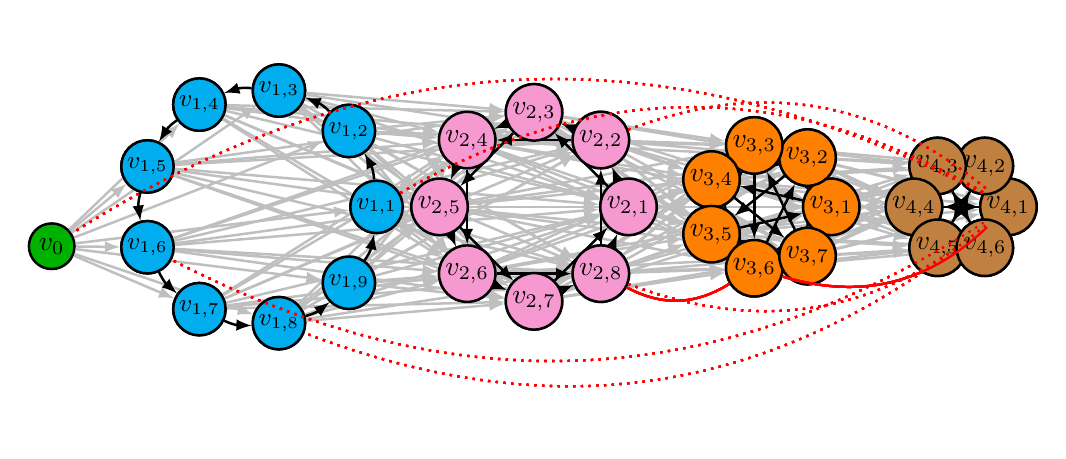
\begin{tikzpicture}[>=latex, line width=0.9pt]
		% --- 2. Nodes (Main Layer) ---
		% R0 Parent
		\node[fill=green!70!black,draw, circle, inner sep=2pt] (v0) at (0, -0.5) {\(v_0\)};
		% R1 Cycle Nodes
		\def\n{9} \def\radius{1.5} \def\centerx{3.5}
		\foreach \i in {1,...,\n} {
			\node[fill=cyan, draw, circle, inner sep=1.2pt] (v1\i) at ({0.75*\centerx + \radius*cos(360/\n*(\i-1))}, {\radius*sin(360/\n*(\i-1))}) {\small \(v_{1,\i}\)};
		}
		% R2 Cycle Nodes
		\def\m{8} \def\rradius{1.2}
		\foreach \i in {1,...,\m} {
			\node[fill=magenta!40,draw, circle, inner sep=1.2pt] (v2\i) at ({1.75*\centerx + \rradius*cos(360/\m*(\i-1))}, {\rradius*sin(360/\m*(\i-1))}) {\(v_{2,\i}\)};
		}
		% R3 Cycle Nodes
		\def\p{7} \def\rrradius{0.8}
		\foreach \i in {1,...,\p} {
			\node[fill=orange,draw, circle, inner sep=1.2pt] (v3\i) at ({2.6*\centerx + \rrradius*cos(360/\p*(\i-1))}, {\rrradius*sin(360/\p*(\i-1))}) {\(v_{3,\i}\)};
		}
		% R4 Cycle Nodes
		\def\q{6} \def\rrradius{0.6}
		\foreach \i in {1,...,\q} {
			\node[fill=brown,draw, circle, inner sep=1.2pt] (v4\i) at ({3.3*\centerx + \rrradius*cos(360/\q*(\i-1))}, {\rrradius*sin(360/\q*(\i-1))}) {\(v_{4,\i}\)};
		}
		
		% --- 3. Arcs (Background Layer) ---
		% Arcs from R0 to R1
		\foreach \i in {1,...,\n} {
			\draw[lightgray,->] (v0) -- (v1\i);
		}
		
		% Arcs from R1 to R2
		\foreach \i in {1,...,\n}{
			\foreach \j in {1,...,\m} {
				\draw[lightgray,->] (v1\i) -- (v2\j);
			}
		}
		
		% Arcs from R2 to R3
		\foreach \i in {1,...,\m}{
			\foreach \j in {1,...,\p} {
				\draw[lightgray,->] (v2\i) -- (v3\j);
			}
		}
		
		% Arcs from R3 to R4
		
		\foreach \i in {1,...,\p}{
			\foreach \j in {1,...,\q} {
				\draw[lightgray,->] (v3\i) -- (v4\j);
			}
		}
		
		% R1 Interior Arcs
		\foreach \i [evaluate=\i as \next using {int(mod(\i,\n)+1)}] in {1,...,\n} {
			\draw[->, bend right=15] (v1\i) to (v1\next);
		}
		
		% R2 Interior Arcs
		\foreach \i [
		evaluate=\i as \next using {int(mod(\i,\m)+1)},
		evaluate=\i as \anext using {int(mod(\i+1,\m)+1)}] in {1,...,\m} {
			\draw[->] (v2\i) to (v2\next);
			\draw[->] (v2\i) to (v2\anext);
		}
		
		% R3 Interior Arcs
		\foreach \i [
		evaluate=\i as \next using {int(mod(\i,\p)+1)},
		evaluate=\i as \anext using {int(mod(\i+1,\p)+1)},
		evaluate=\i as \aanext using {int(mod(\i+2,\p)+1)}] in {1,...,\p} {
			\draw[->] (v3\i) to (v3\next);
			\draw[->] (v3\i) to (v3\anext);
			\draw[->] (v3\i) to (v3\aanext);	
		}
		
		% R4 Interior Arcs
		\foreach \i [
		evaluate=\i as \next using {int(mod(\i,\q)+1)},
		evaluate=\i as \anext using {int(mod(\i+1,\q)+1)},
		evaluate=\i as \aanext using {int(mod(\i+2,\q)+1)},
		evaluate=\i as \aaanext using {int(mod(\i+3,\q)+1)}] in {1,...,\q} {
			\draw[->] (v4\i) to (v4\next);
			\draw[->] (v4\i) to (v4\anext);
			\draw[->] (v4\i) to (v4\aanext);
			\draw[->] (v4\i) to (v4\aaanext);	
		}
		
		% R1 Cycle Nodes
		\def\n{9} \def\radius{1.5} \def\centerx{3.5}
		\foreach \i in {1,...,\n} {
			\node[fill=cyan, draw, circle, inner sep=1.2pt] (v1\i) at ({0.75*\centerx + \radius*cos(360/\n*(\i-1))}, {\radius*sin(360/\n*(\i-1))}) {\small \(v_{1,\i}\)};				
		}
		
		% R2 Cycle Nodes
		\def\m{8} \def\rradius{1.2}
		\foreach \i in {1,...,\m} {
			\node[fill=magenta!40,draw, circle, inner sep=1.2pt] (v2\i) at ({1.75*\centerx + \rradius*cos(360/\m*(\i-1))}, {\rradius*sin(360/\m*(\i-1))}) {\(v_{2,\i}\)};	
		}
		% R3 Cycle Nodes
		\def\p{7} \def\rrradius{0.8}
		
		\foreach \i in {1,...,\p} {
			\node[fill=orange,draw, circle, inner sep=1.2pt] (v3\i) at ({2.6*\centerx + \rrradius*cos(360/\p*(\i-1))}, {\rrradius*sin(360/\p*(\i-1))}) {\(v_{3,\i}\)};	
		}
		
		% R3 Cycle Nodes
		\def\q{6} \def\rrradius{0.6}
		\foreach \i in {1,...,\q} {
			\node[fill=brown,draw, circle, inner sep=1.2pt] (v4\i) at ({3.3*\centerx + \rrradius*cos(360/\q*(\i-1))}, {\rrradius*sin(360/\q*(\i-1))}) {\(v_{4,\i}\)};
			
			
			% \draw[thick, dotted, red] (v41) to [bend left](v0);
			
			\draw[thick, dotted, red] (v41) to [bend right](v0);
			\draw[thick, dotted, red] (v41) to [bend right](v11);
			\draw[thick, dotted, red] (v41) to [bend left](v16);
			\draw[thick, dotted, red] (v41) to [bend left](v18);
			\draw[thick, dotted, red] (v41) to [bend right](v22);
			\draw[thick, dotted, red] (v41) to [bend left](v28);
			\draw[thick, solid, red] (v28) to [bend right](v36);
			\draw[thick, solid, red] (v36) to [bend right](v41);
		}
	\end{tikzpicture}
	\caption{\textit{\textbf{Visualization of Girth)}. Brooks's Equitable Coloring forces Seymour nodes to balance distribution of back arcs. These are spread across neighborhoods until they reach $k-2$ where a triangle is formed. For simplicity, dotted back back arcs only shown from $v_{4,1}$. Triangle is bold red $v_{4, 1} \to v_{2, 8} \to v_{3, 6} \to v_{4_1}$. } } \label{caccimage}
\end{figure}


\begin{conjecture}[CH]
	Every simple directed graph with $n$
	vertices and a minimum outdegree $\delta^+ \ge r$ contains a directed cycle of length at most $\lceil n/r \rceil$
\end{conjecture}

\begin{corollary}
	An oriented graph with minimum outdegree $\delta$. $\lceil n/r \rceil$. In particular, the existence of a Seymour vertex implies the existence of a triangle.
\end{corollary}
\begin{proof}
	The Reduction Theorem \ref{red} prevents back arcs before the Seymour vertices.
	The binomial theorem does not allow these Seymour vertices to have all their arcs through standard neighborhood decreasing. Instead, back arcs must come into place to compensate.
	%		To prevent earlier neighborhoods from having a Seymour vertex in an MCE,
	To ensure that all Seymour vertices meet their degree requirements, Brooks's equitable coloring principle must be applied.
	This says that no Seymour vertex can send back arcs to more than $|R_k| / 3$ nodes in the neighborhood $R_i$ for $R_1$ through $R_{k-2}$.
	
	This will exhaust the $\delta$ for every Seymour vertex. Once we reach the penultimate neighborhood of $R_{k-2}$, a triangle is reached. This proves that the girth of the graph cannot exceed 3. 	
\end{proof}

\section{Acknowledgments}
I am deeply thankful to God for the inspiration and guidance that shaped this work, as Proverbs 3:5-6 has been a guiding light throughout this journey. I am profoundly grateful to my family—my wife and children, my mother, and father—for their unwavering support and encouragement.

Special thanks to the late Dr. Nate Dean and Dr. Michael Ball for their contributions and support to this work. I want to sincerely thank everyone who has taken the time to pray for me, share encouraging words, and offer constructive feedback. Your support has meant so much to me, and I’m truly grateful for the kindness and thoughtfulness you’ve shown.

I also appreciate the Department of Mathematics at Morehouse College for helpful discussions that were valuable during the research process. In particular, I thank Dr. Duane Cooper for asking the questions regarding understanding the conjecture, my approach and how cycles are important.

Finally, I extend heartfelt gratitude to my family and friends for their patience and belief in me throughout this journey.

%\end{desc}
%% --------------------------------------------------------------------
% Bibliography
%% --------------------------------------------------------------------
%		\bibliographystyle{acm}
%\bibliography{references.bib}
\begin{thebibliography}{99}
	
	\bibitem{AMMref} N. Alon, C. McDiarmid, and M. Molloy, Edge-disjoint cycles in regular directed graphs, \emph{J. Combin. Theory Ser. B} \textbf{66} (1996), 273--278.
	
	\bibitem{BMN} Botler, F., Moura, P., and Naia, T. (2022). Seymour's Second Neighborhood Conjecture for orientations of (pseudo)random graphs. \textit{Discrete Mathematics}, 346.
	
	\bibitem{BBKS} Brantner, J., Brockman, G., Kay, B., and Snively, E. (2009). Contributions to Seymour's second neighborhood conjecture. \textit{Involve}, 2(4), 387--395.
	
	\bibitem{CHref} Caccetta, L; H\"{a}ggkvist, R. On minimal digraphs with given girth. Proceedings of the Ninth Southeastern Conference on Combinatorics, Graph Theory, and Computing (Florida Atlantic Univ., Boca Raton, Fla., 1978), pp. 181--187, Congress. Numer., XXI, Utilitas Math., Winnipeg, Man., 1978.
	
	\bibitem{CS} Chen, G., Shen, J., and Yuster, R. (2003). Second Neighborhood via First Neighborhood in Digraphs. \textit{Annals of Combinatorics}, 6, 15--20.
	
	\bibitem{Da} Daamouch, M. (2021). Seymour's second neighborhood conjecture for m-free, k-transitive, k-anti-transitive digraphs and some approaches. \textit{Discrete Appl. Math.}, 304, 332--341.
	
	\bibitem{daamouch2024secondneighborhoodconjecturetournaments} Daamouch, Moussa and Ghazal, Salman and Al-Mniny, Darine, About the second neighborhood conjecture for tournaments missing two stars or disjoint paths, arXiv:2406.03635, 2024.
	
	\bibitem{DL} Dean, N., and Latka, B. (1995). Squaring the tournament-an open problem. \textit{Proceedings of the 26th Southeastern International Conference on Combinatorics}, 73--80.
	
	\bibitem{Di} Díaz, A. E., Girão, A., Granet, B., and Kronenberg, G. (2024). Seymour's second neighbourhood conjecture: random graphs and reductions. \textit{arXiv preprint arXiv:2403.02842}.
	
	\bibitem{D} Diestel, Reinhard, Graph Theory, Springer, 2005.
	
	\bibitem{FidlerYuster} Fidler, D., and Yuster, R. (2007). Remarks on the second neighborhood problem. \textit{J. Graph Theory}, 55(3), 208--220.
	
	\bibitem{F} Fisher, D. C. (1996). Squaring a tournament: A proof of Dean's conjecture. \textit{J. Graph Theory}, 23(1), 43--48.
	
	\bibitem{Ghazal_2011} Ghazal, S., Seymour's second neighborhood conjecture for tournaments missing a generalized star, J. Graph Theory, 71, 89--94, 2012.
	
	\bibitem{GodsilRoyle2001} Godsil, Chris D. and Royle, Gordon F., Algebraic Graph Theory, Springer, 2001
	
	\bibitem{HKPS} Hassan, Z.R., Khan, I.F., Poshni, M.I., and Shabbir, M., Seymour's second neighborhood conjecture for 6-antitransitive digraphs, Discrete Applied Mathematics, 292, 59--63, 2021.
	
	\bibitem{HT} Havet, F., and Thomassé, S. (2000). Median orders of tournaments: A tool for the second neighborhood problem and Sumner's conjecture. \textit{J. Graph Theory}, 35, 244--256.
	
	\bibitem{HP} Huang, H., and Peng, F. (2024). An improved bound on Seymour's second neighborhood conjecture. \textit{arXiv preprint arXiv:2412.20234}.
	
	\bibitem{J} Jungnickel, D, Graphs, networks and algorithms, Springer-Verlag, 2005
	
	\bibitem{KL} Kaneko, Y., and Locke, S. (2001). The minimum degree approach for Paul Seymour's distance 2 conjecture. \textit{Congressus Numerantium}, 148, 201--206.
	
	\bibitem{Llado2013} Lladó, A. (2013). On the second neighborhood conjecture of Seymour for regular digraphs with almost optimal connectivity. \textit{European Journal of Combinatorics}, 34(8), 1265--1271.
	
	\bibitem{MninyGhazal} Mniny, D. A., and Ghazal, S. (2020). The Second Neighborhood Conjecture for oriented graphs missing $\{C_{4}, \overline{C_{4}}, S_{3}, \text{chair and co-chair}\}$-free graph. \textit{arXiv:2010.10790}.
	
	\bibitem{NALYVAIKO2021poster} Nalyvaiko, I. (2021). Properties of possible counterexamples to the Seymour's Second Neighborhood Conjecture. \textit{Poster presented at the EUCYS 2020/2021 Contest}.
	
	\bibitem{Scrt} Seacrest, T. (2019). Seymour's Second Neighborhood Conjecture for Subsets of Vertices \textit{arXiv:1808.06293v3}
\end{thebibliography}

\end{document}
